\section{Research Protocol}
\label{sec:hpath-protocol}

This section presents the experimental setup for the case studies to answer our research questions. The goal of this chapter is to analyze the impact of using second-generation locators relying on rendered features. Thus, we rely on two main concepts: the properties of an element HPath can leverage to generate a query and its resilience to changes happening during the \gls{sut} evolution. In this study, the properties are measured by the length of the location path and the presence of predicates in any step of the location path. The resilience to change of a locator is evaluated by its propensity to avoid breakage following a change in the \gls{html} document.

\subsection{Projects Collection}
\label{sec:hpath-protocol-projects}

To select adequate projects for a case study, we mine repositories from Github, using its search \gls{api} which allows to apply queries to filter the result from the Github database. Because of the restrictions of the mining process described in Section~\ref{sec:hpath-protocol-elements}, we have to isolate projects with tests written in Java and exercising the Selenium \gls{api}. Furthermore, both application code and test code need to be versioned in the same repository to be able to go back in time and run test suites for previous versions.

Moreover, because of the dynamic nature of our analysis, we need to be able to compile the projects and run them on successive versions. Unfortunately, despite our best effort, most of the projects we gathered could not be executed in our experimental setup (missing dependencies, outdated build tools). Thus, this process yields two large web based open-source systems: OpenOLAT\footnote{https://github.com/OpenOLAT/OpenOLAT}, a web-based e-learning platform and MISO LIMS\footnote{https://github.com/miso-lims/miso-lims}, a lab information management system designed for tracking next-generation sequencing experiments. Both projects rely on a Java backend that is communicating with a \gls{rdbms}. For the front end, both use \gls{html}, CSS and Javascript however MISO LIMS is relying on the HTML4 standard while OpenOLAT is using the \gls{html}5 standard. Finally, both project adopt a multi-tier architecture relying on different services working in concert.

\begin{table}
\centering
\caption{Web Applications used in our experiments. Column \emph{\#Releases} presents the number of releases collected, \emph{KLoC} is the number of thousand lines of code in the last release, \emph{\#Tests} is the rounded average number of integration tests per release and \emph{\#Locators} is the total number of locators recorded.}
\label{tab:hpath-protocol-projects}
\begin{tabular}{>{\raggedright}m{0.7in}>{\raggedleft}m{0.7in}>{\raggedleft}m{0.7in}>{\raggedleft}m{0.7in}>{\raggedleft}m{0.7in}}
\toprule
\textbf{\scriptsize{Project}} & \textbf{\scriptsize{\#Releases}} & \textbf{\scriptsize{KLoC}} & \textbf{\scriptsize{\#Tests}} & \textbf{\scriptsize{\#Locators}} \tabularnewline
\toprule
\scriptsize{\textit{OpenOLAT}} & \scriptsize{8} & \scriptsize{1308} & \scriptsize{154} & \scriptsize{216424} \tabularnewline
\scriptsize{\textit{MISO LIMS}} & \scriptsize{57} & \scriptsize{326} & \scriptsize{8} & \scriptsize{15672} \tabularnewline
\bottomrule
\end{tabular}
\end{table}

Table~\ref{tab:hpath-protocol-projects} presents some key metrics of the projects under study. The 57 versions of MISO LIMS were collected between March 2019 and November 2020 and the 8 versions of OpenOLAT span from November 2018 to August 2020. 

The low number of versions for the OpenOLAT project (8 versions) is due to the fact that earlier versions could not be compiled (Maven Plugin not supported). While both projects are quite large in terms of lines of code, we can see that the developers of the project MISO LIMS do not rely heavily on \gls{gui}-based testing, with an average number of 8 tests per version.

\begin{figure}
\centering
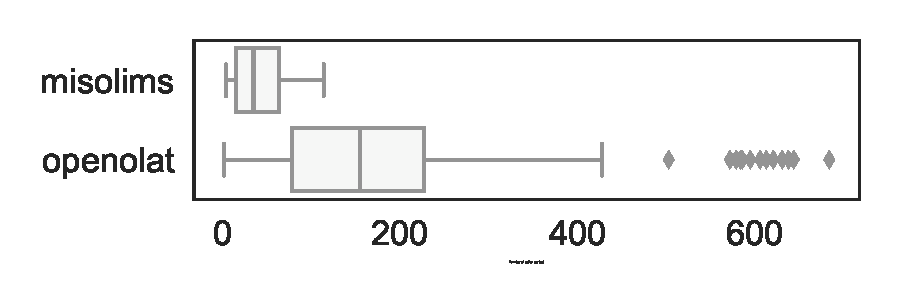
\includegraphics[width=0.8\columnwidth]{figures/hpath/selector-per-test-dist.pdf}
\caption{Number of actions triggered by test.}  
\label{fig:hpath-protocol-actions}
\end{figure}

Figure~\ref{fig:hpath-protocol-actions} presents the number of actions triggered by the tests for each project under study. In average, the number of actions triggered by a test is 170 for the OpenOLAT project and about 42 for the MISO LIMS project. One intriguing point shown by the figure is the presence of tests not containing any interaction with the application through Selenium. These are tests not targeting the \gls{sut} through the user interface but rather directly interacting with the \gls{api} of the application or the \gls{rdbms} itself, thus falling out of the purview of \gls{suit}s.

\subsection{Mining Locator Breakages}
\label{sec:hpath-protocol-elements}

We developed a tool called Mercator\footnote{Available at \url{https://github.com/UL-SnT-Serval/mercator}} to capture the state of the pages and the \gls{dom}-based locators used to interact with it in the test suites. 

\subsubsection{Selenium Instrumentation}
\label{sec:hpath-protocol-instrumention}

More specifically, Mercator instruments method calls \emph{findElement} and \emph{findElements} from the class \emph{RemoteWebDriver} offered by the Selenium \gls{api}. Hence, at runtime, Mercator captures the following data every time a test exercises a \gls{dom}-based locator: (1) information about the state of the current web page \ie\ complete dump of the \gls{dom}, size of the window and current \gls{url}; (2) information about the test \ie\ test name, call stack, inference on the previous call stack; (3) information about the locator \ie\ locator strategy, locator value; (4) information about the project \ie\ repository \gls{url}, commit id, previous commit id, commit date. This process is repeated for each version defined in the configuration of Mercator. For this study, we select every release of the projects. We restrict our study to releases because the projects rely on external dependencies which are not stable during the development cycle, thus, leading to code that cannot compile due to missing dependencies (SNAPSHOT). Furthermore, using releases increases the chances of observing genuine \gls{sut} evolution, thus, reduces noise.

\subsubsection{HTML Dump}
\label{sec:hpath-protocol-capture}

The most sensitive aspect of this process is collecting the \gls{dom} dumps. Indeed, as explained in Section~\ref{sec:hpath-introduction-HTML}, a \gls{html} document can contain links to other resources such as multimedia and \gls{css} style sheet stored externally. Thus, for the dump to be usable as a single \gls{html} document file, during the instrumentation, a complete \gls{html} document with no external dependencies needs to be computed. This is done by inlining all the \gls{css} style sheets in the header, and providing placeholders for all multimedia content retaining their attributes, size and position. Furthermore, all properties computed by JavaScript are inlined in the style attribute of the elements and all script elements are removed from the dump. This is possible because pages are captured after the execution of all JavaScript routines which may alter the structure of the \gls{dom} tree. Finally, comment nodes and any formatting of the \gls{html} document not affecting its content (line returns between to subsequent elements) are removed to limit syntactic differences between dumps.

One caveat encountered during instrumentation is the non-negligible amount of time (between 200ms to up to 1500ms during our experiments depending on the complexity of the page) required to create the dump. This delay causing tests to run slower might break some which are bounded by a maximum time budget (\emph{timeout}). This leads us to use a strategy to monitor changes in the \gls{dom} tree to minimize the number of time the state has to be computed. Unfortunately, this changes failed to detect changes not altering the tree but modifying external properties of the elements (mostly hovering and selections in table) which lead to generating locators in our dataset that are not valid, 20.09\% for MISO LIMS and 8.57\% for OpenOLAT. We deem this tradeoff reasonable compared to the alternative where we observe about 35\% of the tests failing due to our instrumentation.

With reasonable performance when instrumenting one version, the next step consist in devising a strategy to compute the lineage of a locator across versions. To achieve this objective, we rely on the change log computed by the versioning system Git. Mercator enriches the data it records (locator and \gls{dom}) with information about the version and the test that is currently running. Then using the current stack trace and the change log between the current version and the previous version (identified by their commit IDs) it is able to offer an approximation of the stack trace in the previous commit. To do so, it recomputes the stack trace in the previous version, taking into account line additions and deletions in the test code. This process is described in details in Section~\ref{sec:hpath-protocol-pairs}.

Finally, the last step of this process is the extraction of the elements themselves. Each data point generated by Mercator contains a locator and its associated HTML document. Thus, by querying the \gls{dom} with the collected locators, we can retrieve the elements targeted by the tests relying on Selenium. The Selenium API offers different strategies to locate web elements that are shown in Table~\ref{tab:selenium_strategies}. 

\begin{table}
\centering
\caption{Element selection strategies defined by the Selenium API.}
\label{tab:selenium_strategies}
\begin{tabular}{>{\raggedright}m{1in}>{\raggedright}m{3in}}
\toprule
\textbf{\scriptsize{Strategy}} & \textbf{\scriptsize{Description}}\tabularnewline
\toprule
\scriptsize{\textit{class name}} & \scriptsize{Locates elements whose class attribute contains the search value.} \tabularnewline
\scriptsize{\textit{css selector}} & \scriptsize{Locates elements matching the CSS selector.} \tabularnewline
\scriptsize{\textit{id}} & \scriptsize{Locate elements whose id attribute matches the search value.} \tabularnewline
\scriptsize{\textit{link text}} & \scriptsize{Locates anchor elements, $E_a$, whose inner text matches the search value.} \tabularnewline
\scriptsize{\textit{patial link text}} & \scriptsize{Locates anchor elements, $E_a$, whose inner text contains the search value.} \tabularnewline
\scriptsize{\textit{tag name}} & \scriptsize{Locates elements whose tag name matches the search value.} \tabularnewline
\scriptsize{\textit{xpath}} & \scriptsize{Locates elements matching the location path.} \tabularnewline
\bottomrule
\end{tabular}
\end{table}

\subsubsection{Pairs Creation}
\label{sec:hpath-protocol-pairs}

As shown in Figure~\ref{fig:hpath-protocol-actions}, each test exercises a large number of actions and simply relying on test name does not offer the granularity required for this analysis. Thus, we rely on \emph{stack traces} to uniquely identify an element query in a version. The \emph{stack trace} is the stack of subroutine state information from the test entry point to Selenium API call to locate an element. Each subroutine call is defined by a fully qualified class name, a method name and a line number. Unfortunately, this method is sensitive to changes in the test code base from one version to another. Indeed, if lines are added or deleted before the call, then the line number is affected. Furthermore, when classes or methods are renamed, the subroutine information of the corresponding frame is modified. To minimize this effect, we compute the \emph{previous stack trace} which is the stack trace that a call would have had in the previous version when accounting from the change extracted from the \emph{unified diff} obtained through the version control system. We recompute the line number based on the line additions and deletions that occurred before the call in the file. If the target line is modified or there are class or method name changes, then, we consider that no mapping is possible. At this stage, each call to Selenium API can be identify by a \emph{stack trace} and is associated to a \emph{previous stack trace}. Thus, to create the pairs we link calls qualified by a tuple $<stack\:traces,\:version>$ to calls with a matching tuple $<previous\:stack\:traces,\:previous\:version>$. We will call $version_A$ and $version_B$, the first version and the next version of the pair respectively.

\subsubsection{Breakage Detection}
\label{sec:hpath-protocol-breakage-detection}

Once the pairs are created, we filter out any pair not exhibiting a \gls{sut} evolution. For each \gls{dom} we compute a hash code based on its string representation. Then, we filter out any pair where $hash_A = hash_B$ thus only accounting for pairs containing changes in the \gls{dom}. We consider a locator to break following a change in $<DOM_A, DOM_B>$, if querying $DOM_B$ with $locator_A$ returns an empty set, \emph{i.e.} fails to locate any element. We perform this operation on all pairs of the dataset where $hash_A \neq hash_B$. This process leads to a total of 30,436 pairs.

\subsection{RQ1: Target Elements}
\label{sec:hpath-protocol-rq1}

The approach that we propose, HPath, makes the assumption that the interactions with the \gls{html} document mainly targets visible elements, \emph{i.e.} elements rendered on the web page. 

Indeed, under our hypothesis, a test should interact with elements to navigate through the states of the web application then make assertions on visible elements to validate the proper execution of the test as a human would. Thus, not all elements of the \gls{html} document hold the same value for the testers. To assess this hypothesis and answer RQ1, we extract the type (tags) of the elements targeted by the tests. Comparing this distribution with the one contained in the \gls{html} document, we can assess which elements SUITs typically interact with. 

Furthermore, previous work targets elements systematically\cite{Cohen2015, Leotta2015, Aldalur2017, Eladawy2018} or generates test scripts\cite{Grechanik2009, Montoto2011, Kirinuki2019} when a \gls{gui} test suite is not available. Unfortunately, studies relying on \emph{in vivo} \gls{gui} test suites are usually conducted on industrial projects and the source code is not available\cite{Thummalapenta2013, Yandrapally2014}. While there exists studies tackling the question of the evolution and the characteristics of \gls{gui} tests \cite{Christophe2014}, they usually rely on static analysis and do not convey information about locators and their target elements. Thus, understanding which type of elements are targeted by testers would allow researchers to create benchmarks to evaluate their approaches by following the same distributions observed in other projects when no tests are available.

\subsection{RQ2: Element Properties Used by Locators}
\label{sec:hpath-protocol-rq2}

To evaluate HPath, we compare it against two approaches to generate XPath: absolute XPath and Robula+. We select XPath algorithms because our approach is a derivative of XPath with the aim of addressing one of its limitation: its reliance on structural properties of the \gls{html} document, making HPath more flexible to changes of the internal document structure.

The first algorithm, absolute XPath, builds an XPath where each step can only rely on a positional predicate. Thus, it does not rely on any attributes such as id, class or name and can be seen as the most naive form of XPath generation. Note that when using the absolute XPath algorithm, the deeper an element is nested in a \gls{dom} tree, the longer the location path. Thus, this algorithm tends to leak the overall structure of the \gls{dom}, where any change in the node hierarchy of target elements will alter its absolute XPath representation.

Robula+ \cite{Leotta2016} is a state-of-the-art XPath generation algorithm developed by the research community. The aim behind this algorithm is to generate robust XPath locators. It works with the assumption that the shorter the location path is, the less it leaks the overall structure of the \gls{dom}, thus making it more robust to changes in the \gls{dom} hierarchy. To generate the shortest location path possible, the algorithm starts with (\texttt{//*}), which selects every node, $N_D$, and then refine the expression in consecutive specialization steps until only the target candidate can be selected by the expression, $N_{target} \subseteq N_D$. Each refinement step is based on heuristics to improve the expressiveness and robustness of the final location path. During the refinement steps, the heuristics define the order in which Robula+ tries to select an attribute to build a predicate\footnote{We follow the recommendations from the authors: \emph{name}, \emph{class}, \emph{title}, \emph{alt}, \emph{value}.} and the attributes to ignore\footnote{We follow recommendations from the authors: \emph{href}, \emph{src}, \emph{onclick}, \emph{onload}, \emph{tabindex}, \emph{width}, \emph{height}, \emph{style}, \emph{size}, \emph{maxlength}.}.

Note that other algorithms to generate robust XPath locators have been proposed in the literature, notably \textcite{Montoto2011, Thummalapenta2013}. The two alternative algorithms rely on similar properties as Robula+ (id, name, class) but are less robust\cite{Leotta2016}. As for other approaches relying on a combination of XPath and other strategies\cite{Leotta2015, Aldalur2017}, they are considered out of scope since HPath could be integrated in such approaches. Furthermore, we consider third-generation approaches out of scope, because of their reliance on computer vision techniques which in itself bring a new set of challenges.

To characterize the properties exploited by the different approaches we proceed in two phases. First, we compute the length (number of steps) of the location paths generated by the three approaches. Indeed, previous work consider the addition of extra nodes in the location path as increasing the fragility of the path. For example, \textcite{Leotta2015} introduce the fragility coefficient as a function of the number of node traversed and in Chapter~\ref{chap:smells-system-user-interactive-test} we observe the SUIT smell sensitive locator which qualify as bad practice to have any location path traversing more than one node.

Then, we conduct a fine-grain analysis of the predicates that are used by Robula+ and HPath (absolute XPath is omitted since it does not compute predicates). The goal here is to show which properties of the \gls{dom} elements can be exploited by the two approaches.

\subsection{RQ3: Locators Resilience to SUT Evolution}
\label{sec:hpath-protocol-rq3}

Finally, we analyze which locators manage to successfully retrieve the element in the next version. In the cases of locator breakage, we perform a fine-grain analysis to isolate the cause of the breakage. This analysis is based on the structure of the location path where each step is composed of a node test and an optional predicate. Therefore, we compare $locator_A$ and $locator_B$ from the breaking pairs and extract their difference. The cause of the breakage is based on the type of changes observed between the two location paths. For example, if $locator_A$ is //div[@id="old"] and $locator_B$ is //div[@id="new"], then the cause of the breakage is classified as \emph{predicate id attr.}. The list of all breakage causes is presented in Table~\ref{tab:breakage_cause}. 